\chapter{Application : recherche de bugs dans Radare2}

Afin de mettre en application le fuzzing avec AFL, nous avons ciblé le logiciel Radare2 (logiciel libre disponible sur github\footnote{\url{https://github.com/radare/radare2}}) afin de découvrir de potentiels problèmes dans celui-ci.
Radare2 est un logiciel de reverse-engineering open-source et développé activement par une large communauté.
Il s'agit d'ailleurs d'une suite d'outils (radare2, rasm2, rax2, rafind2...) permettant entre autre de désassembler des binaires pour un nombre important d'architectures (x86, ARM, MIPS...), d'obtenir des informations sur de nombreux formats (ELF, PE, MACHO...), etc.

Nous avons décidé de cibler Radare2 étant donné qu'il possède une surface d'attaque assez importante et qu'il s'agit d'un logiciel de plus en plus utilisé dans le domaine du reverse-engineering \cite{radare2}.

\section{Address Sanitizer (ASan)}

Avant de parler de méthodologie, il est nécessaire de présenter un outil développé par Google permettant de détecter un certain nombre de problèmes de corruptions mémoire.
Cet outil, ASan pour ``Address Sanitizer'', est actuellement implémenté pour les compilateurs Clang, GCC et Xcode.
Il permet lorsque l'on compile un programme en C ou C++ de rajouter de l'instrumentation au binaire qui va vérifier à l'exécution que l'on n'accéde pas à des zones mémoires qui ne seraient pas autorisées dans un comportement normal du logiciel.
ASan permet ainsi de détecter les problèmes suivants :

\begin{itemize}
\item heap/stack overflows (read et write out-of-bounds) ;
\item overflows dans des buffers situés dans .data ou .bss ;
\item use-after-free ;
\item double-free ;
\item etc.
\end{itemize}

À savoir que ASan ne détecte pas tous les problèmes de corruption comme par exemple les lectures de mémoire non initialisée, les overflows dans des buffers situés dans des structures, ou encore des corruptions de mémoire arbitraire comme lorsqu'un integer overflow a lieu pour calculer le décalage de l'accès mémoire.

Pour compiler un programme avec ASan, il suffit par exemple de fournir l'option \lstinline{-fsanitize=address} à \lstinline{gcc} ou \lstinline{clang} pour que celui-ci compile en rajoutant l'instrumentation de ASan au programme.

Comme vous le constaterez en lisant les sections suivantes, l'avantage de ASan est de détecter des problèmes de sécurité qui seraient restés silencieux lors d'une utilisation normale du programme.
Par contre, ASan n'est pratiquement pas utilisé en production étant donné que l'instrumentation rajoute une augmentation des temps d'exécution de 73\% et une utilisation de la mémoire de 340\% en moyenne \cite{asan}.

\section{Méthodologie}

Notre approche concernant le fuzzing de Radare2 s'est déroulé comme suit :

\begin{itemize}
\item Récupération des sources et compilation de AFL ;
\item Récupération des sources de Radare2, et compilation de celui-ci avec \lstinline{afl-gcc} afin d'instrumenter le programme ;
\item Compréhension de la suite d'outils de Radare2, ciblage des entrées utilisateur et écriture des jeux de tests ;
\item Lancement de plusieurs instances d'AFL sur nos jeux de tests précédents ;
\item Analyse des crashs obtenus et des différentes mutations avec ASan.
\end{itemize}

\subsection{Installation de AFL}

Pour récupérer les sources de AFL, il suffit de se rendre sur le site de lcamtuf\footnote{\url{http://lcamtuf.coredump.cx/afl/releases/afl-latest.tgz}} pour récupérer l'archive, et de compiler le fuzzer en tapant simplement \lstinline{make} une fois le zip décompressé.

\subsection{Instrumentation de Radare2 grâce à \emph{afl-gcc}}

Nous avons compilé deux versions de Radare2 : une version normale instrumentée avec \lstinline{afl-gcc} et une autre compilée avec ASan afin de découvrir de nouveaux problèmes.
La première version peut se compiler de cette manière :

\begin{lstlisting}
  $ git clone https://github.com/radare/radare2.git radare2
  $ mkdir radare2-install
  $ cd radare2
  $ CC=path-to-afl-gcc ./sys/user.sh --install-path ../radare2-install
\end{lstlisting}

Pour obtenir une version compilée avec ASan, nous pouvons utiliser ces commandes :

\begin{lstlisting}
  $ git clone https://github.com/radare/radare2.git radare2-asan
  $ mkdir radare2-install-asan
  $ cd radare2-asan
  $ ASAN=address ./sys/asan.sh -u --install-path ../radare2-install-asan
\end{lstlisting}

Il faut savoir que ASan peut difficilement être utilisé avec AFL.
En effet, en moyenne, l'instrumentation effectuée par ASan multiplie par 3.4 la mémoire utilisée par le programme\cite{asan}, alors que AFL essaie de limiter la quantité de mémoire utilisée pendant le fuzzing d'un programme pour préserver la stabilité du système.
Pour pouvoir l'utiliser avec AFL il aurait été nécessaire de le compiler en 32bits, ce que nous n'avons pas réussi à faire sur les serveurs du CREMI.

\subsection{Écriture des entrées initiales pour le fuzzing}

Maintenant, il est nécessaire de choisir quelles sont les parties de Radare2 que nous souhaitons tester avec AFL.
Nous avons tenté de fuzzer les composants suivants :

\begin{itemize}
\item radare2 : il s'agit du programme principal du projet Radare2.
  Celui-ci peut prendre en paramètre des scripts exécutant des commandes et un fichier binaire à analyser.

  Nous avons choisi de tester à la fois le parsing des scripts passés à radare2, et à la fois le parser des formats de fichiers binaires.
\item rasm2 : il s'agit d'un programme permettant de désassembler des instructions codées en hexadécimal passées dans un fichier.
\item rax2 : une calculatrice supportant plusieurs bases (binaire, hexadécimal).
\item rafind2 : un outil permettant de donner des informations sur le type de fichier passé en paramètre (à la manière de la commande \lstinline{file}).
\item rabin2 : un outil pouvant donner différentes informations sur le fichier binaire passé en paramètre (sections, segments...).
\end{itemize}

Pour fuzzer les formats de fichiers, nous avons utilisé les dépôts binary-sample\footnote{\url{https://github.com/JonathanSalwan/binary-samples}} et radare2-regressions\footnote{\url{https://github.com/radare/radare2-regressions}} en utilisant les binaires les plus petits de chaque format afin d'accélérer le fuzzing.

Pour les outils \lstinline{rasm2}, \lstinline{rax2} et \lstinline{radare2} (partie scripts), nous avons simplement écrit un fichier valide minimal de quelques octets pour chaque outil.

\subsection{Lancement de \emph{afl-fuzz}}

Une fois tout ce travail effectué, nous avons lancé une instance de \lstinline{afl-fuzz} pour chaque partie du logiciel testé.
Pour cela, nous avons utilisé les serveurs de calculs (\path{mcgonagall.emi.u-bordeaux.fr}) mis à disposition du CREMI possédant pas moins de 48 CPUS AMD64 et 128 Go de mémoire RAM.
Après environ trois jours, nous avons obtenu un certains nombre de crashs grâce à nos jeux de tests et AFL.

Chaque instance de AFL peut être lancée de la manière suivante, où le dossier \path{in/} contient nos jeux de tests initiaux.
Par exemple, pour fuzzer les scripts de radare2 :

\begin{lstlisting}
  $ ./radare2/env.sh ./radare2-install
  $ afl-fuzz -i in -o out -m 256M ./radare2-install/bin/radare2 -i @@ -q /sbin/ebtables
\end{lstlisting}

Ici, les caractères '@@' seront remplacés par le fichier muté par AFL, c'est à dire le script initial du dossier \path{in/} avec les modifications appliquées par \lstinline{afl-fuzz}.

Ci-dessous, le résultat d'une des instances de AFL lancée sur l'outil \lstinline{radare2} :

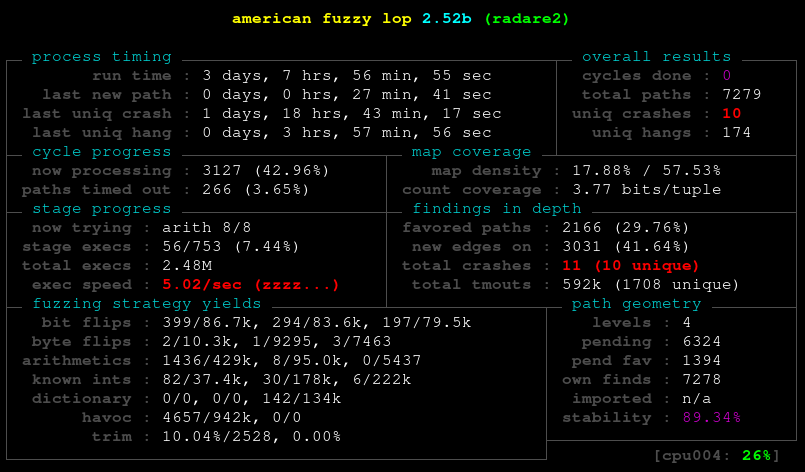
\includegraphics[width=0.9\linewidth]{../medias/afl-fuzz.png}

\subsection{Analyse des résultats obtenus}

Après quelques jours de fuzzing, nous avons obtenus dix crashs sur le parsing des commandes \lstinline{radare2} et un crash sur le parsing des fichiers binaires (toujours sur l'outil \lstinline{radare2}).
Les fichiers générant ces crashs sont stockés dans le dossier \path{out/crashes/}, les entrées s'exécutant en plus d'une seconde (temps de timeout par défaut de AFL) dans le dossier \path{out/hangs/} et l'ensemble des mutations dans le dossier \path{out/queue/}.

Afin de découvrir d'autres problèmes potentiels, nous avons réexécuté notre version de Radare2 compilée avec ASan sur l'ensemble des fichiers présents dans \path{out/queue/}.
Cela nous a permis de découvrir notamment un problème dans l'outil \lstinline{rax2} et d'autres problèmes dans le parsing des scripts de \lstinline{radare2}.
L'analyse de ces différents problèmes sont présentés dans la section suivante.

\section{Problèmes constatés}

\subsection{radare2 (interpréteur) - read out of bounds}

Nous avons tout d'abord identifié un problème de type ``read out-of-bounds'' sur un buffer situé dans le heap.
Le bug se situe dans l'exécution de la commande \lstinline{dbw} dans l'interpréteur Radare2.
Voici un extrait du log de ASan lorsque l'on exécute cette commande dans Radare2 :

\begin{lstlisting}
  ==30389==ERROR: AddressSanitizer: heap-buffer-overflow on address 0x60200006c694 at pc 0x7f6213972144 bp 0x7ffed25f8010 sp 0x7ffed25f8008
  READ of size 1 at 0x60200006c694 thread T0
  #0 0x7f6213972143 in r_str_trim_ro .../radare2-src-asan/libr/util/str_trim.c:89
  #1 0x7f6219c81e68 in r_core_cmd_bp .../radare2-src-asan/libr/core/cmd_debug.c:3361
  ...
\end{lstlisting}

Si on analyse le code de la fonction \lstinline{r_str_trim_ro} dans le fichier \path{libr/util/str_trim.c}, nous constatons qu'il s'agit simplement d'un code permettant d'avancer le pointeur de la chaîne passée en paramètre jusqu'au prochain caractère n'étant pas un espace :

\begin{lstlisting}[language=C]
R_API const char *r_str_trim_ro(const char *str) {
  if (str) {
    for (; *str && IS_WHITECHAR (*str); str++) {
      ;
    }
  }
  return str;
}
\end{lstlisting}

Le problème se situe dans la fonction \lstinline{r_core_cmd_bp} qui s'occupe d'analyser les commandes commençant par 'd'\footnote{Le code est commenté par nos soins pour se focaliser sur le bug et ne pas perdre le lecteur. Cette remarque est valable pour l'ensemble du code présenté dans cette partie.} :

\begin{lstlisting}[language=C]
  /* ... */
  case 'w': // "dbw"
      input++; // skip 'w'
      watch = true;
      // passthru
  case ' ': ;// "db"
      #define DB_ARG(x) r_str_word_get0(str, x)
      char *str = strdup (r_str_trim_ro (input + 2));
  /* ... */
\end{lstlisting}

On voit ici que le troisième caractère est comparé à travers un switch-case et que si la commande est ``dbw'', le pointeur \lstinline{input} est incrémenté : il pointe maintenant sur la chaîne ``w''.
Le problème, c'est qu'il n'y a pas de \lstinline{break} à la fin de ce \lstinline{case}, ce qui fait que le deuxième \lstinline{case} est également exécuté.
On voit alors que la fonction \lstinline{r_str_trim_ro} est appliqué sur un buffer situé un caractère en dehors de la chaîne.

\subsection{radare2 (interpréteur) - double free}

Un ``double free'' est également présent dans cette même fonction (\lstinline{r_core_cmd_bp}).
Le bug se situe dans le morceau de code suivant :

\begin{lstlisting}[language=C]
case ' ': ;// "db"
  #define DB_ARG(x) r_str_word_get0(str, x)
  char *str = strdup (r_str_trim_ro (input + 2));
  int i = 0;
  int sl = r_str_word_set0 (str);

  for ( ; i < sl; i += 1 + (watch ? 1 : 0)) {
    if (*DB_ARG(i) == '-') {
      /* ... */
    } else {
      if (watch) {
        if (sl % 2 == 0) {
          if (!strcmp (DB_ARG (i + 1), "r")) {
            rw = R_BP_PROT_READ;
          } else if (!strcmp (DB_ARG (i + 1), "w")) {
            /* ... */
          } else {
            r_core_cmd_help (core, help_msg_dbw);
            /* free 1 */
            free (str);
            break;
          }
        } else {
          r_core_cmd_help (core, help_msg_dbw);
          /* free 1-bis */
          free (str);
          break;
        }
      }
      /* ... */
    }
  }
  /* free 2 */
  free (str);
  break;

case 'i':
  /* ... */

\end{lstlisting}

Dans cette portion de code, les arguments situés après la commande \lstinline{dbw} sont parcourus.
Si le deuxième argument n'est ni ``r'', ``w'' ou ``rw'' (free 1) ou que le nombre d'arguments est impair (free 1-bis) le pointeur \lstinline{str} est free une fois et on sort de la boucle avec le \lstinline{break}.
Ici le développeur voulait sans doute sortir du \lstinline{switch} également, mais un deuxième \lstinline{free} est appliqué sur ce même pointeur (free 2) : nous avons une vulnérabilité de type ``double free''.

On peut par exemple taper dans \lstinline{radare2} la commande \lstinline{dbw a a} ou \lstinline{dbw r r r} pour déclencher le bug.
Un morceau de la trace généré par ASan au moment du ``double free'' :
\begin{lstlisting}
  ==31123==ERROR: AddressSanitizer: attempting double-free on 0x60200006c610 in thread T0:
  #0 0x7fcaf8889a10 in free (/usr/lib/x86_64-linux-gnu/libasan.so.3+0xc1a10)
  #1 0x7fcaf7e5760a in r_core_cmd_bp .../radare2-src-asan/libr/core/cmd_debug.c:3416

  freed by thread T0 here:
  #0 0x7fcaf8889a10 in free (/usr/lib/x86_64-linux-gnu/libasan.so.3+0xc1a10)
  #1 0x7fcaf7e5763a in r_core_cmd_bp .../radare2-src-asan/libr/core/cmd_debug.c:3384
\end{lstlisting}

\subsection{radare2 (interpréteur) - bad pointer dereference}

Nous avons également découvert une erreur de segmentation due à une erreur de type dans une chaîne de format.
Le problème peut être constaté lorsque l'on tape \lstinline{aa} suivi de \lstinline{pifjA} dans l'outil \lstinline{radare2} :

\begin{lstlisting}
  ==2181==ERROR: AddressSanitizer: SEGV on unknown address 0x000000000041 (pc 0x7f36f2a795b2 bp 0x7ffd4cb07950 sp 0x7ffd4cb07088 T0)
  #0 0x7f36f2a795b1  (/usr/lib/x86_64-linux-gnu/libasan.so.3+0xd85b1)
  #1 0x7f36f2a2b731  (/usr/lib/x86_64-linux-gnu/libasan.so.3+0x8a731)
  #2 0x7f36f2a2d61d in __interceptor_vsnprintf (/usr/lib/x86_64-linux-gnu/libasan.so.3+0x8c61d)
  #3 0x7f36f1f95439 in r_core_cmdf .../radare2-src-asan/libr/core/cmd.c:3903
  #4 0x7f36f20692b4 in cmd_print .../radare2-src-asan/libr/core/cmd_print.c:4496
  ...
\end{lstlisting}

Si on analyse la fonction \lstinline{cmd_print} à l'endroit du segfault, nous voyons ceci :

\begin{lstlisting}[language=C]
case 'f': // "pif"
  if (input[2] == '?') { // "pif?"
    /* ... */
  } else if (input[2] == 'j') {
    r_core_cmdf (core, "pdfj%s", input[3]);
  } else if (input[2] == 'c') { // "pifc"
\end{lstlisting}

Ici, \lstinline{input[3]} est de type \lstinline{char} alors que le format ``\%s" attend un type \lstinline{char*}.
Le caractère sera alors considéré comme l'adresse à afficher.
En effet, ici cette chaîne de caractère est directement passée à \lstinline{vsnprintf} comme l'on peut le constater si l'on regarde la fonction \lstinline{r_core_cmdf} :

\begin{lstlisting}[language=C]
R_API int r_core_cmdf(RCore *core, const char *fmt, ...) {
  char string[4096];
  int ret;
  va_list ap;
  va_start (ap, fmt);
  vsnprintf (string, sizeof (string), fmt, ap);
  ret = r_core_cmd (core, string, 0);
  va_end (ap);
  return ret;
}
\end{lstlisting}

\subsection{radare2 (parser PE) - double free}

Nous avons trouvé une vulnérabité de type ``double free'' dans le parser du format PE (Portable Executable). Il est en effet possible de construire un fichier PE contenant deux noms de ressources, pointant au même endroit. Le problème se situe dans la fonction \lstinline{_parse_resource_directory} :

\begin{lstlisting}[language=C]
static void _parse_resource_directory(struct PE_(r_bin_pe_obj_t) *bin, Pe_image_resource_directory *dir, ut64 offDir, int type, int id, HtUU *dirs, char *resource_name) {
  /* ... */

  for (index = 0; index < totalRes; index++) {
    /* ... */
    ut8 *resourceEntryName = NULL;
    if (entry.u1.s.NameIsString) { /* [1] */
      /* ... */
      resourceEntryName = calloc (resourceEntryNameLength + 1, sizeof (ut8));
      /* ... */
    }

    if (entry.u2.s.DataIsDirectory) { /* [2] */
      /* ... */
      if (resource_name && resourceEntryName) {
        /* ... */
        R_FREE (resource_name);
      }
      /* [3] */
      _parse_resource_directory (bin, &identEntry,
        entry.u2.s.OffsetToDirectory, type, entry.u1.Id, dirs, (char *)resourceEntryName);
      continue;
    }

    /* ... */
    r_pe_resource *rs = R_NEW0 (r_pe_resource);
    /* ... */
    if (resource_name) { /* [4] */
      rs->name = resource_name;
    } else {
      char numberbuf[6];
      rs->name = strdup (sdb_itoa (id, numberbuf, 10));
    }
    r_list_append (bin->resources, rs);
  }
}
\end{lstlisting}

Pour arriver à une telle erreur, il faut un PE contenant une ressource de type directory tout en passant par [1] pour allouer le \lstinline{resource_name} et par [2] pour effectuer un appel récursif avec un \lstinline{resource_name} différent de \lstinline{NULL} en [3].
Ensuite, cette ressource de type directory doit contenir deux entrées : \lstinline{resource_name} étant différent de \lstinline{NULL}, le \lstinline{rs->name} de chaque entrée pointera alors sur la même zone mémoire [4].

Lorsque l'on quitte \lstinline{radare2}, la fonction \lstinline{_free_resources} est appelée sur chacune de nos deux entrées :

\begin{lstlisting}[language=C]
static void _free_resources(r_pe_resource *rs) {
  if (rs) {
    free (rs->name);
    /* ... */
  }
}
\end{lstlisting}

On déclenche alors un ``double free'' comme le montre le message de ASan suivant :

\begin{lstlisting}
  ==19003==ERROR: AddressSanitizer: attempting double-free on 0x631000028800 in thread T0:
  #0 0x7f678602ca10 in free (/usr/lib/x86_64-linux-gnu/libasan.so.3+0xc1a10)
  #1 0x7f6784464350 in _free_resources .../radare2-src-asan/libr/..//libr/bin/p/../format/pe/pe.c:1218
  #2 0x7f677f1ad4c5 in r_list_delete .../radare2-src-asan/libr/util/list.c:107
  #5 0x7f67844a5e7f in Pe32_r_bin_pe_free .../radare2-src-asan/libr/..//libr/bin/p/../format/pe/pe.c:3526

  0x631000028800 is located 0 bytes inside of 65536-byte region [0x631000028800,0x631000038800)
    freed by thread T0 here:
    #0 0x7f678602ca10 in free (/usr/lib/x86_64-linux-gnu/libasan.so.3+0xc1a10)
    #1 0x7f6784464350 in _free_resources .../radare2-src-asan/libr/bin/format/pe/pe.c:1218
\end{lstlisting}


\subsection{rax2 (calculatrice hexa) - use after free}

Un problème de type ``use-after-free'' a été découvert dans l'outil \lstinline{rax2} grâce à ASan.
AFL n'ayant à priori pas trouvé de crash lors de son exécution, nous avons en effet décidé de relancer la version de \lstinline{rax2} compilé avec ASan sur l'ensemble des entrées générées par le fuzzer.

Sur une de ces entrée, nous avons obtenu le message suivant :

\begin{lstlisting}
  ==6459==ERROR: AddressSanitizer: heap-use-after-free on address 0x60200000eff6 at pc 0x7f806a1b1129 bp 0x7ffd36d90400 sp 0x7ffd36d903f8
  READ of size 1 at 0x60200000eff6 thread T0
  #0 0x7f806a1b1128 in cin_get .../radare2-src-asan/libr/util/calc.c:220
  #1 0x7f806a1b1128 in get_token .../radare2-src-asan/libr/util/calc.c:263
  #2 0x7f806a1b2794 in prim .../radare2-src-asan/libr/util/calc.c:140
  #3 0x7f806a1b1630 in term .../radare2-src-asan/libr/util/calc.c:108
  #4 0x7f806a1b207c in expr .../radare2-src-asan/libr/util/calc.c:88
  #5 0x7f806a1b31a6 in r_num_calc .../radare2-src-asan/libr/util/calc.c:406
  #6 0x7f806a0fbbc3 in r_num_math .../radare2-src-asan/libr/util/unum.c:412
  ...
  freed by thread T0 here:
  #0 0x7f806a903a10 in free (/usr/lib/x86_64-linux-gnu/libasan.so.3+0xc1a10)
  #1 0x7f806a0fc035 in r_num_tailff .../radare2-src-asan/libr/util/unum.c:762
\end{lstlisting}

Nous observons alors que la commande \lstinline{echo "0xF..1" | rax2} est à l'origine de ce message.
Le principal problème se situe dans la fonction \lstinline{r_num_tailff}, appelée lorsqu'elle rencontre une chaîne de type "0xF.." :

\begin{lstlisting}[language=C]
static ut64 r_num_tailff(RNum *num, const char *hex) {
  char *p;
  int i;
  /* ... */
  p = malloc (strlen (hex) + 10);
  if (p) {
    /* ... */
    if (isxdigit ((ut8)hex[0])) {
      n = r_num_math (num, p);
    } else {
      /* ... */
    }
    free (p);
  }
  /* ... */
}
\end{lstlisting}

Ici, le pointeur \lstinline{p} est passé à la fonction \lstinline{r_num_math}, puis \lstinline{free} à la suite.
Le problème, c'est que ce pointeur est assigné au champ \lstinline{num->nc->calc_buf} lors de \lstinline{r_num_math} :

\begin{lstlisting}[language=C]
static void load_token(RNum *num, RNumCalc *nc, const char *s) {
  /* ... */
  nc->calc_buf = s;
  /* ... */
}
\end{lstlisting}

Plus tard, lors du traitement du token "1" de notre chaîne de caractère, la fonction \lstinline{cin_get} est exécutée :

\begin{lstlisting}[language=C]
static int cin_get(RNum *num, RNumCalc *nc, char *c) {
  /* ... */
  *c = nc->calc_buf[nc->calc_i];
  /* ... */
}
\end{lstlisting}

Ici, le buffer \lstinline{nc->calc_buf} pointe vers une adresse qui a été libérée dans notre fonction \lstinline{r_num_tailff} : nous déclenchons un ``use-after-free'' en lecture.

\paragraph{}
L'ensemble de ces problèmes ont été remontés à l'équipe de Radare2 et corrigés.
Le tableau ci-dessous résume l'ensemble des bugs trouvés et analysés lors de ce projet avec un lien vers l'issue et le commit corrigeant celui-ci\footnote{Certains bugs de ce tableau ne sont pas présentés dans ce rapport car ils ont été trouvés et signalés ultérieurement. De plus, cela aurait certainement allourdi la lecture de celui-ci.}

\paragraph{}
\begin{tabularx}{\textwidth}{|r|c|X|c|c|}
    \hline
    \textbf{Outil} & \textbf{Code impacté} & \textbf{Classe de bug} & \textbf{Issue} & \textbf{Commit} \\
    \hline
    radare2 & interpréteur & read out-of-bounds & \href{https://github.com/radare/radare2/issues/13031}{\#13031} & \href{https://github.com/radare/radare2/commit/ce73397}{ce73397} \\
    \hline
    radare2 & interpréteur & double free & \href{https://github.com/radare/radare2/issues/13032}{\#13032} & \href{https://github.com/radare/radare2/commit/26baccd}{26baccd} \\
    \hline
    radare2 & interpréteur & bad pointer dereference & \href{https://github.com/radare/radare2/issues/13033}{\#13033} & \href{https://github.com/radare/radare2/commit/4cdc50f}{4cdc50f} \\
    \hline
    radare2 & parser PE & double free & \href{https://github.com/radare/radare2/issues/13035}{\#13035} & \href{https://github.com/radare/radare2/commit/868bda4}{868bda4} \\
    \hline
    rax2 & calculatrice hexa & use after free & \href{https://github.com/radare/radare2/issues/13039}{\#13039} & \href{https://github.com/radare/radare2/commit/b4504f9}{b4504f9} \\
    \hline
    radare2 & analyseur ARcompact & read out-of-bounds & \href{https://github.com/radare/radare2/issues/13070}{\#13070} & \href{https://github.com/radare/radare2/commit/5cd5ac3}{5cd5ac3} \\
    \hline
    radare2 & parser Java Class & NULL pointer dereference & \href{https://github.com/radare/radare2/issues/13069}{\#13069} & \href{https://github.com/radare/radare2/commit/3c654cf}{3c654cf} \\
    \hline
    radare2 & parser Java Class & read out-of-bounds & \href{https://github.com/radare/radare2/issues/13067}{\#13067} & \href{https://github.com/radare/radare2/commit/c3339b8}{c3339b8} \\
    \hline
    radare2 & parser PE & stack overflow & \href{https://github.com/radare/radare2/issues/13062}{\#13062} & \href{https://github.com/radare/radare2/commit/56f5eaf}{56f5eaf} \\
    \hline
    radare2 & analyseur Dalvik & bad integer conversion & \href{https://github.com/radare/radare2/issues/13072}{\#13072} & \href{https://github.com/radare/radare2/commit/29eba0a}{29eba0a} \\
    \hline

\end{tabularx}
